\documentclass[12pt]{article}
\usepackage{amsmath, amssymb}
\usepackage{enumitem}
\usepackage{hyperref}
\usepackage{pdfpages}
\usepackage{graphicx}

\title{Applied Math 205, Fall 2024: Problem Set 1}
\author{}
\date{Due: Monday, September 16, 2024, 3:00 PM}

\begin{document}

\maketitle

\section*{Instructions}
Please submit your solutions as a PDF file on Gradescope before the deadline. Concise but mathematically precise answers are encouraged. Code listings must be included in your write-up where applicable. 

\emph{I used ChatGPT 4o for this and supporting code is in the jupiter notebook at the end of the document.}

\section*{Problems}

\textbf{Floating Point Arithmetic: Assume double IEEE precision.}

\begin{enumerate}

    \item (On paper)
    \begin{enumerate}
        \item What is the next floating-point number after 99? 
        
        We know that in the binary representation, \(99=1.10011 \times 2^6\). The next floating-point number will be determined by performing the smallest increment of the mantissa. So we would flip the 52nd bit of the mantissa from 0 to 1, and then multiply the result by \(2^6\). Therefore, the next floating-point number after 99 is 99.000000000000014210854715202003.
        
        \item Exactly how many floating point numbers are there in the interval \([3/2, 2]\)? 
        
        The first step is to determine what our numbers are: \(\frac{3}{2}=1.5\) and \(2=2.0\). If we want to make this into binary representation, we have 1.5 as \(1.1 \times 2^0\) and 2 as \(1.0 \times 2^1\). There are 52 bits of precision in the mantissa between \(1.0=1.0 \times 2^0\) and \(2.0=1.0 \times 2^1\). But we only need half of that, giving us \(2^{51}\) numbers in the interval \([3/2, 2]\).
        
        \item Exactly how many floating point numbers are there in the interval \([1/2, 2/3]\)? 
        
        The first step is to determine what our numbers are: \(\frac{1}{2}=1.0 \times 2^{-1}\) and \(\frac{2}{3}=1.0101010101010101010101010101010101010101010101010101 \times 2^{-1}\). Note that both numbers share the exponent of -1 and 0.5 starts the floating point numbers with this exponent whereas 1.0 is the first number with the new exponent of 0. Therefore, there are \(2^{52}\) numbers in the interval \([1/2, 1] \equiv [\frac{3}{6}, \frac{6}{6}]\) but we are just interested in the interval \([\frac{3}{6}, \frac{4}{6}]\) which is one third of the total interval. Therefore, there are \(\frac{2^{52}}{3}\) numbers in the interval \([1/2, 2/3]\). 
        
        \item Explain why there must be two different floating point numbers \(a, b \in [3/2, 2]\) whose floating point reciprocals \(1/a\) and \(1/b\) are the same.
        
        When taking the reciprocal of a floating point number, there is an inherent rounding error. Therefore, there are many more than just 2 different numbers in the interval with the same reciprocal.
        
    \end{enumerate}

    \item (On the computer) Write a code that sets \(x\) equal to a vector of a million uniformly distributed random numbers in \([0, 1]\) and computes the vector \(y = 1 - x\), i.e., \(y_j = 1 - x_j\), and then computes \( \sum x_j + \sum y_j \). Repeat this with 20 different random vectors \(x\) and report the errors in the sums. Explain why the simplest bound on the error would be larger than \(10^{-5}\) and why the observed errors are smaller.

The fundamental rule for floating point arithmetic is
\begin{equation}
    \text{fl}(x + y) = (x + y)(1 + \epsilon)
\end{equation}
where \(\epsilon\) is the machine epsilon. Now we want to consider the larger case of
\begin{equation}
    \text{fl}{((x+y)+z)} = ((x + y)(1 + \epsilon) + z)(1 + \epsilon) = (x + y + z + \epsilon(x + y) + z)(1 + \epsilon)
\end{equation}
We can approximate this up to order \(O(\epsilon)\) as
\begin{equation}
    \text{fl}{((x+y)+z)} \approx (x + y + z)(1 + \frac{x+y}{x+y+z}\epsilon + \epsilon)
\end{equation}
Now, we know that that fraction will always be less than one, so we can bound the multiplicative factor
\begin{equation}
    1 + \frac{x+y}{x+y+z}\epsilon + \epsilon < 1 + 2\epsilon
\end{equation}
More generally, if we are summing \(n\) numbers, we have
\begin{equation}
    \text{fl}(\sum_{i=1}^{n} x_i) = \sum_{i=1}^{n} x_i(1 + n\epsilon)
\end{equation}
\(n=10^6\) in this case, but we are performing two summations, so the error would be \(n^2\epsilon = 10^{12}\epsilon\). The machine epsilon is \(10^{-16}\), so the error would be \(10^{-4}\), which is larger than \(10^{-5}\). This was the simplest bound on the error that was suggested in the instructions. However, we observe something much smaller, which relates to the fact that the errors will be arbitrary whether they are to the left or right. Therefore, the errors will cancel out to some extent, leading to the smaller observed error of less than $10^{-10}$.
\end{enumerate}

\textbf{Linear Algebra}

\begin{enumerate}
    \item (On paper)
    \begin{enumerate}
        \item Find a 2x2 matrix \(A\) such that \(A\) is ill-conditioned but has determinant 1.
        
        \begin{equation}
            \begin{pmatrix}
                1000 & 0 \\
                0 & 0.001
            \end{pmatrix}
        \end{equation}

        This matrix has a determinant of 1 and then the singular values are 1000 and 0.001, which results in a large condition number of \(10^6\).
        
        \item Find a 2x2 matrix such that \(\|A\|_F = 5\) and \(\|A\|_2 = 4\).
        
        The Frobenius norm is defined as \(\|A\|_F = \sqrt{\sum_{i=1}^{m} \sum_{j=1}^{n} |a_{ij}|^2}\) and the spectral norm is defined as \(\|A\|_2 = \sqrt{\lambda_{\text{max}}(A^TA)}\) or the largest singular value of \(A\): \(\|A\|_2 = \max(\sigma_1, \sigma_2)\). In order to satisfy the first condition, we can set 
\begin{equation}
    5 = \sqrt{a_{11}^2 + a_{12}^2 + a_{21}^2 + a_{22}^2} \implies 25 = a_{11}^2 + a_{12}^2 + a_{21}^2 + a_{22}^2
\end{equation}
16 and 9 are both the squares of the integers 4 and 3, which collectively add up to 25, as desired. In order to satisfy the second condition, we can choose the matrix
\begin{equation}
    A=\begin{pmatrix}
        4 & 0 \\
        0 & 3
\end{pmatrix}
\end{equation}
When we left multiply it by its transpose, we get
\begin{equation}
    A^TA = \begin{pmatrix}
        4 & 0 \\
        0 & 3
    \end{pmatrix} \begin{pmatrix}
        4 & 0 \\
        0 & 3
    \end{pmatrix} = \begin{pmatrix}
        16 & 0 \\
        0 & 9
    \end{pmatrix}
\end{equation}
The largest eigenvalue of this matrix is 16, which is the square of 4, and the largest singular value of \(A\) is 4, as desired.
        
        \item Find a 2x2 matrix such that \((1, 2)^T \in \text{span}(A)\) but \((2, 1)^T \notin \text{span}(A)\).
        
        \[
        A = \begin{pmatrix}
            1 & 0 \\
            0 & 2
        \end{pmatrix}
        \]
        The vector \((1, 2)^T\) can be expressed as a linear combination of the columns of \(A\), while \((2, 1)^T\) cannot.
        
        \item Find a 2x2 matrix such that \(A \neq A^2\) but \(A^2 = A^3\).
        
        In order to satisfy the first condition come we need to find a matrix that is not idempotent. We can choose the matrix
        \begin{equation}
            A = \begin{pmatrix}
                0 & 1 \\
                0 & 0
            \end{pmatrix}
        \end{equation}
        Then, we have
        \begin{equation}
            A^2 = \begin{pmatrix}
                0 & 1 \\
                0 & 0
            \end{pmatrix} \begin{pmatrix}
                0 & 1 \\
                0 & 0
            \end{pmatrix} = \begin{pmatrix}
                0 & 0 \\
                0 & 0
            \end{pmatrix}
        \end{equation}
        but
        \begin{equation}
            A^3 = \begin{pmatrix}
                0 & 1 \\
                0 & 0
            \end{pmatrix} \begin{pmatrix}
                0 & 1 \\
                0 & 0
            \end{pmatrix} \begin{pmatrix}
                0 & 1 \\
                0 & 0
            \end{pmatrix} = \begin{pmatrix}
                0 & 0 \\
                0 & 0
            \end{pmatrix}
        \end{equation}
        So we have satisfied the condition.
    \end{enumerate}

    \item (On the computer) Perform the experiment described in Figure 1 of the document at \url{people.maths.ox.ac.uk/trefethen/sept23lms.pdf} using your preferred software to compute \(A^{-1}\) for a random matrix \(A\). Report your observations.
    
    I am using Python with NumPy on a MacBook Pro M3. I see similar trends, but I need to take the average for multiple trials of dimension sizes less than $10^3$ to see the $O(n^2)$ trend.

    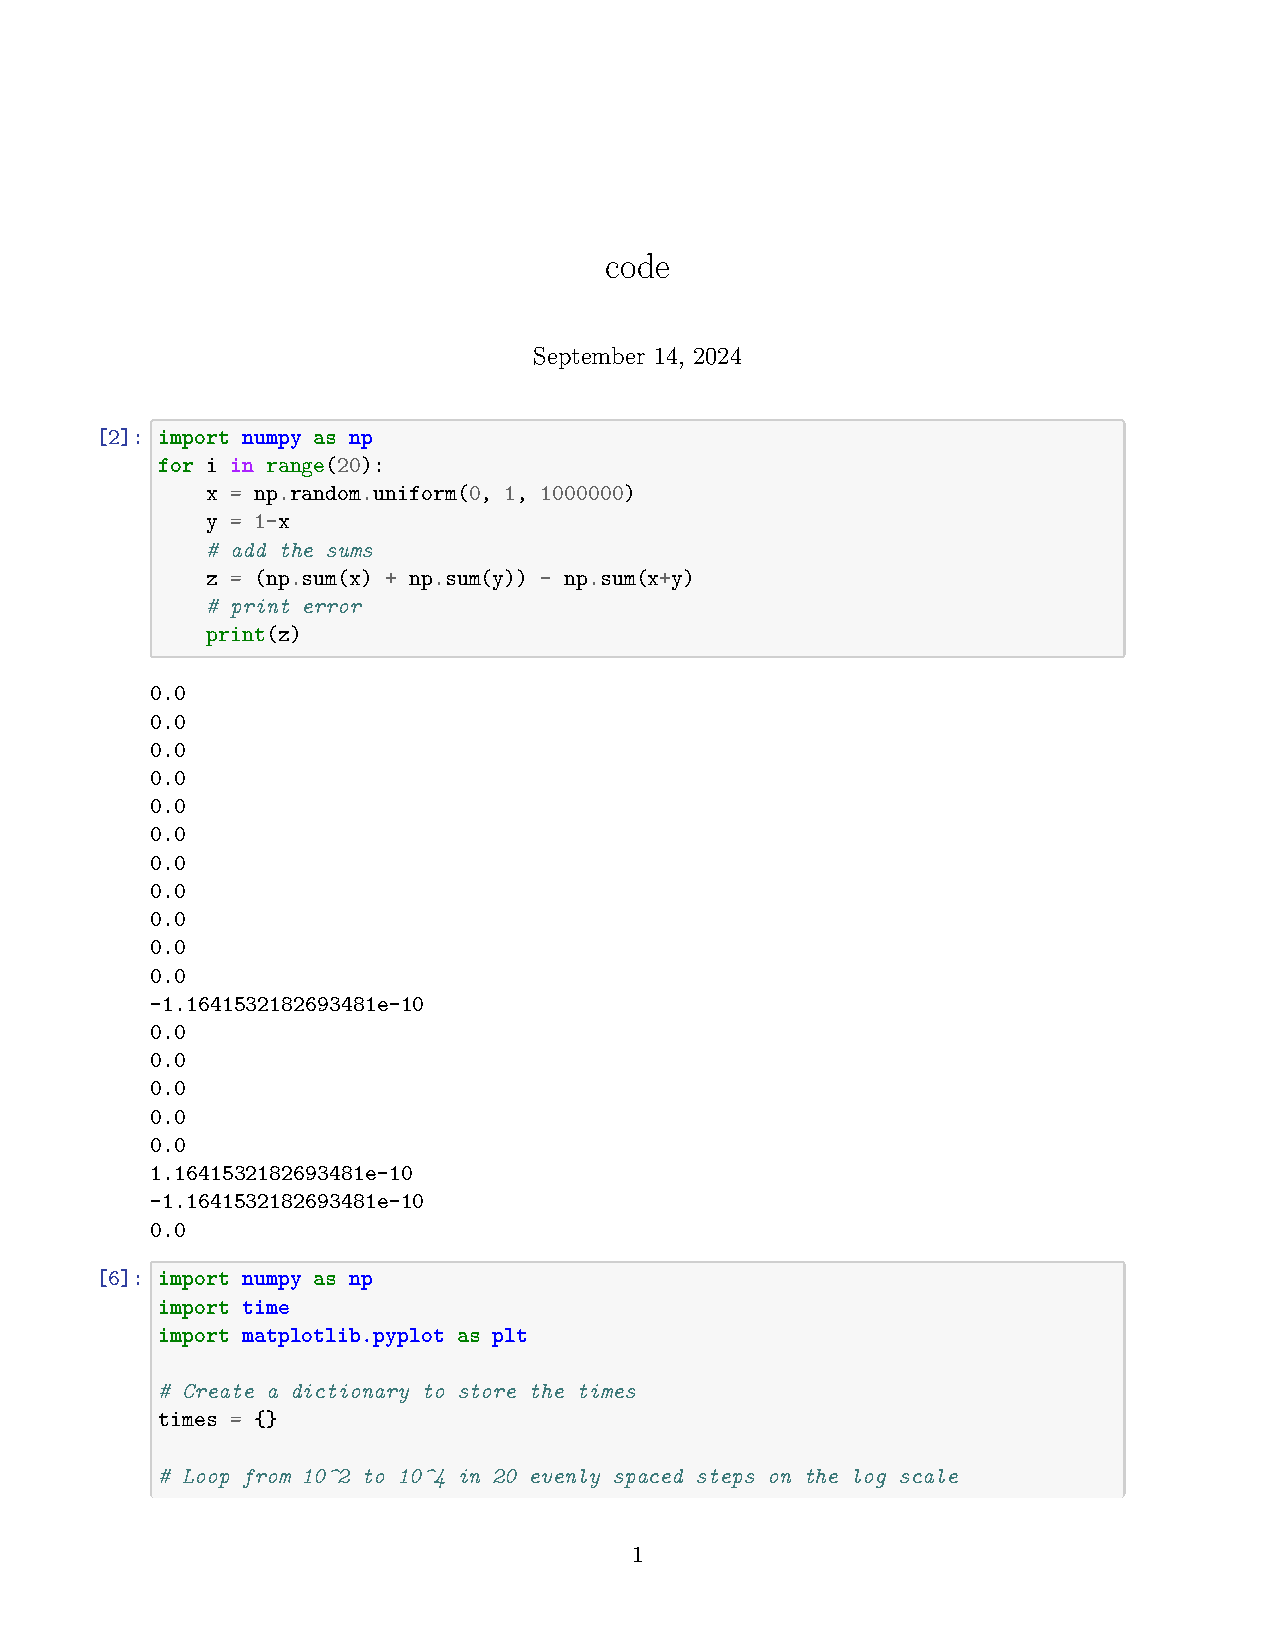
\includepdf[pages=-]{code.pdf}



    
\end{enumerate}

\end{document}
